\begin{landscape}

	\label{uiDrafts} 
	\chapter{User Interface Draft 1}

	\begin{figure}[H]
		\centering
		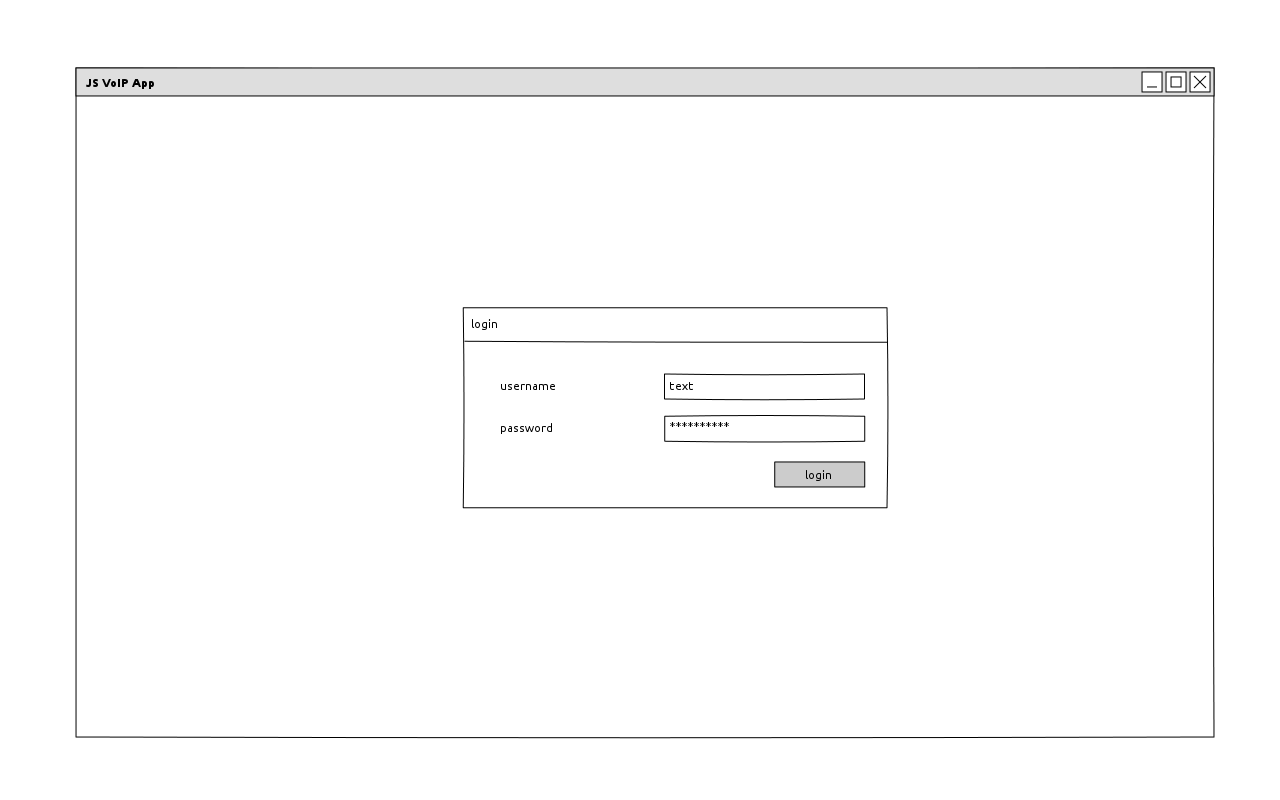
\includegraphics[height=0.6\textwidth]{../ui/img/login_page.png}
		\caption{Über den Login Screen loggen sich Benutzer ein.}
		\label{login screen}
	\end{figure}
	\begin{figure}[H]
		\centering
		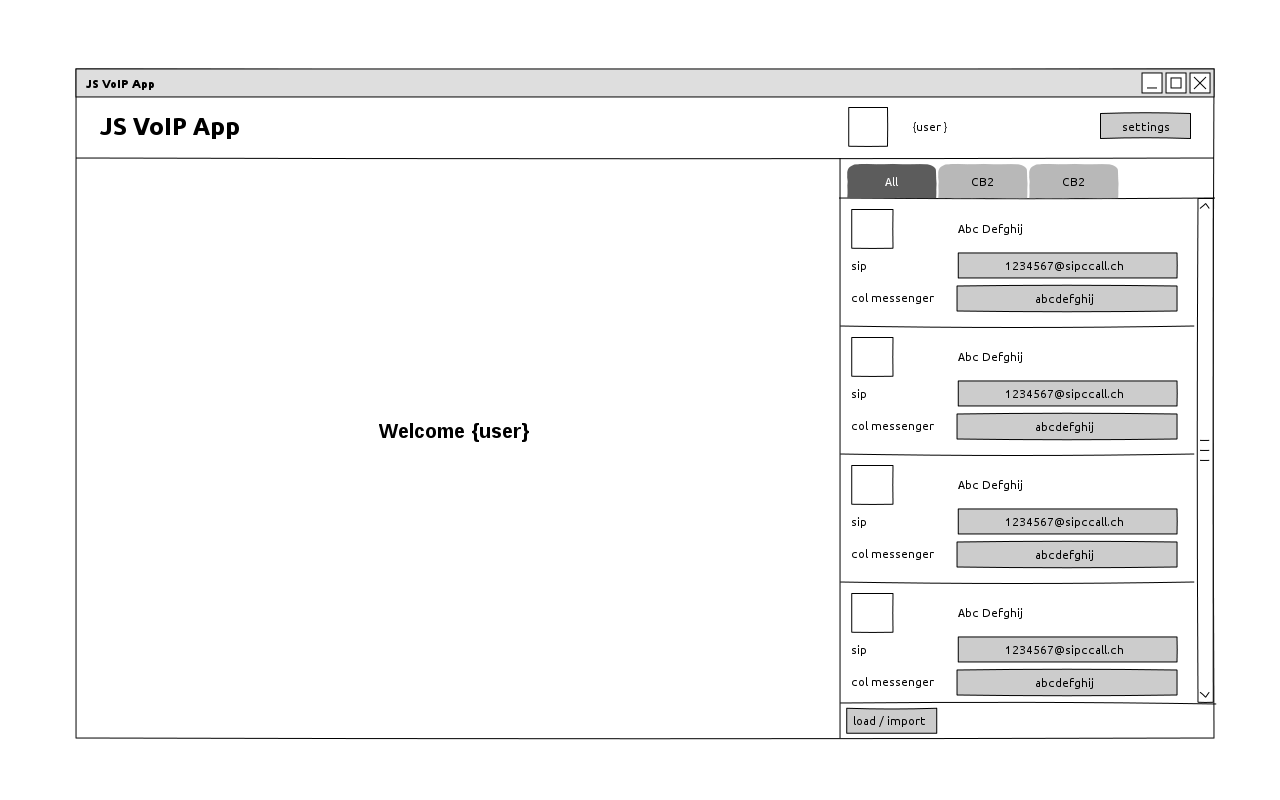
\includegraphics[height=0.8\textwidth]{../ui/img/main_view.png}
		\caption{In der Hauptansicht hat der Benutzer Zugriff auf das Adressbuch.}
		\label{main screen}
	\end{figure}
	\begin{figure}[H]
		\centering
		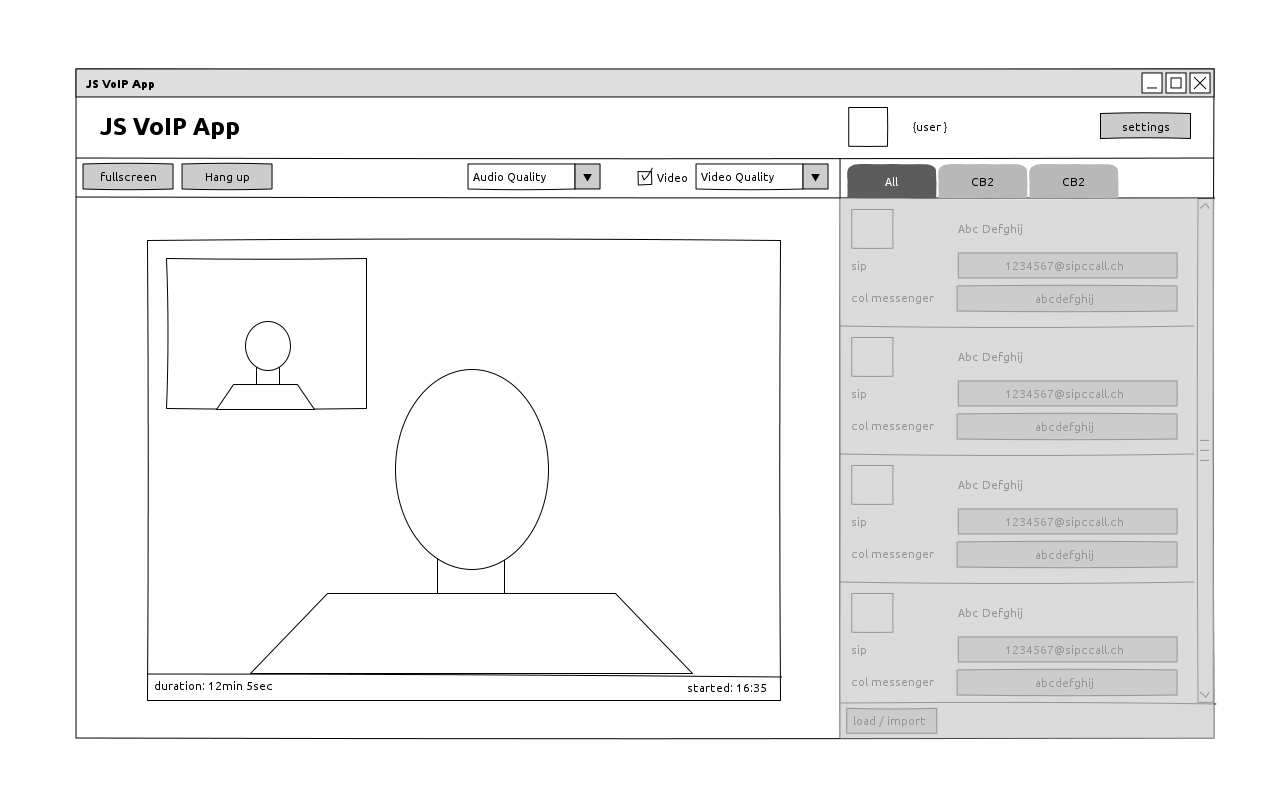
\includegraphics[height=0.75\textwidth]{../ui/img/call_view.png}
		\caption{Ruft der Benutzer einen Kontakt an, so wird das Video in der Hauptansicht eingeblendet und die Kontakte werden inaktiv.}
		\label{call screen}
	\end{figure}
	\begin{figure}[H]
		\centering
		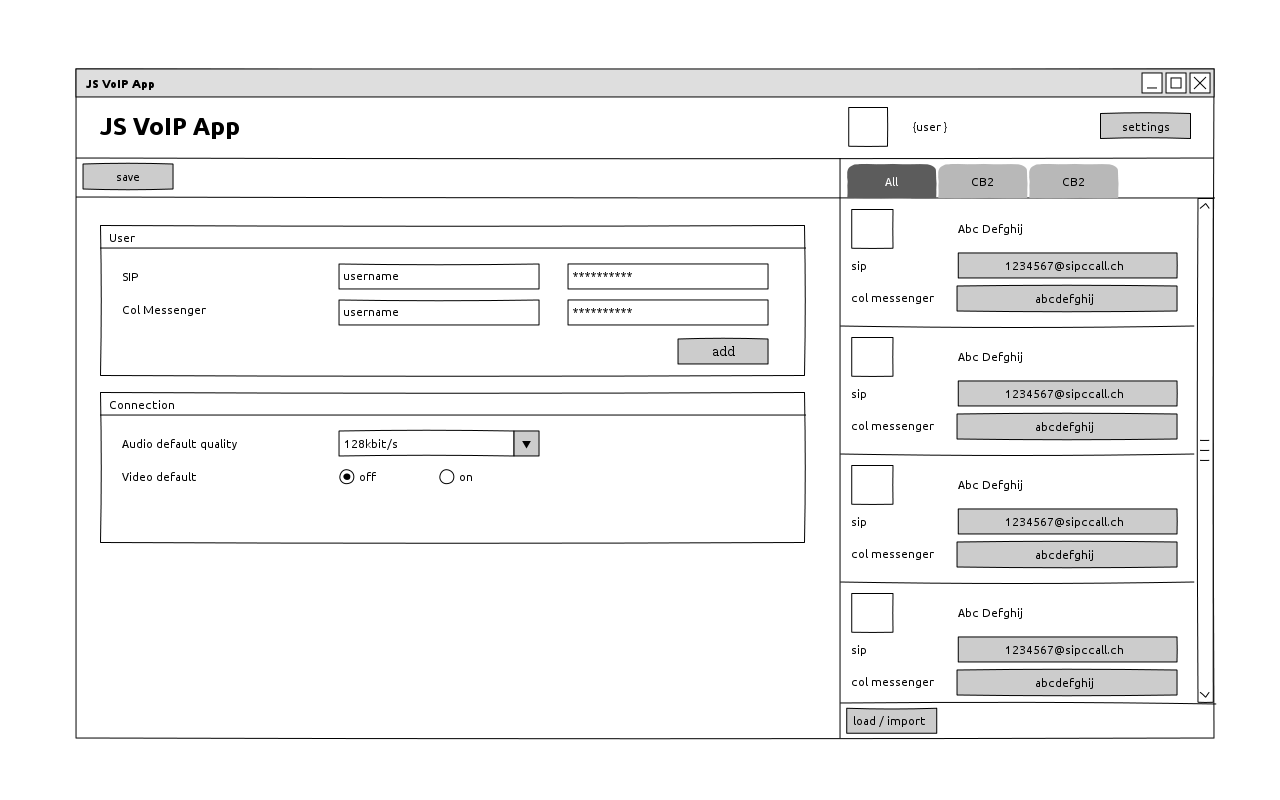
\includegraphics[height=0.75\textwidth]{../ui/img/settings_view.png}
		\caption{Über die Settings kann der Bentzer Einstellungen verändern.}
		\label{settings screen}
	\end{figure}
	
	
\chapter{User Interface Draft 2}
	Das UI2 folgt dem Prinzip ``Mobile First"'.
	\begin{figure}[H]
		\centering
		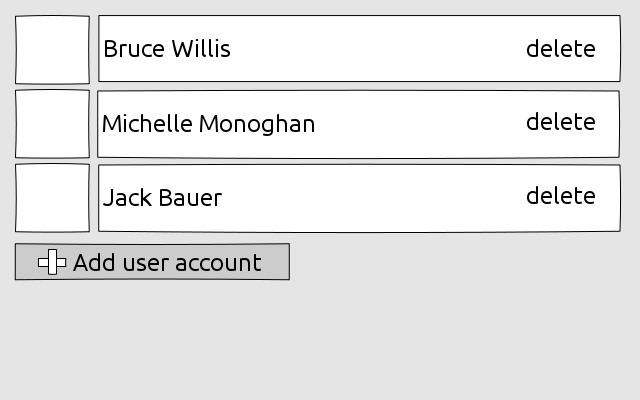
\includegraphics[height=0.6\textwidth]{../ui/img/uiDraft2/UserView-selectUser.png}
		\caption{Benutzer Verwaltung und Login Screen. Durch klick auf einen Benutzer kann sich der Benutzer mit dessen Konto anmelden.}
		\label{login screen}
	\end{figure}
	\begin{figure}[H]
		\centering
		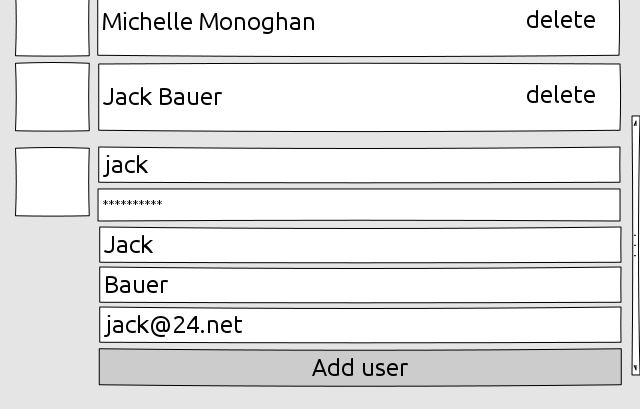
\includegraphics[height=0.6\textwidth]{../ui/img/uiDraft2/UserView-addUser.png}
		\caption{Die Benutzerverwaltung erlaubt es dem benutzer auch gleich einen neuen Bentzer zu erfassen.}
		\label{user management screen}
	\end{figure}
		\begin{figure}[H]
		\centering
		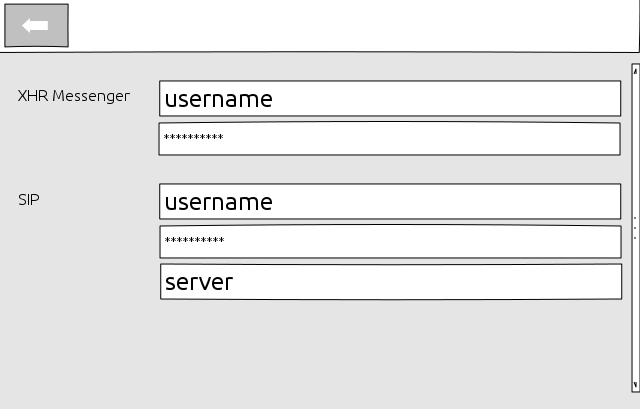
\includegraphics[height=0.6\textwidth]{../ui/img/uiDraft2/UserView-addChannel.png}
		\caption{Die Bentzerverwaltung ermöglicht dem Benutzer das verwalten der verfügbaren Channel Accounts.}
		\label{user management screen}
	\end{figure}
	\begin{figure}[H]
		\centering
		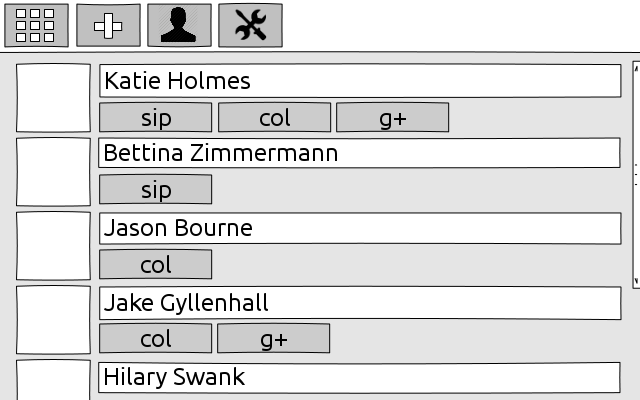
\includegraphics[height=0.6\textwidth]{../ui/img/uiDraft2/ContactbookView.png}
		\caption{Adressbuch: Von hier aus ruft der Benutzer seine Kontakte an. Die verschiedenen Adressbücher sind über das Listensymbol erreichbar.}
		\label{contactbook screen}
	\end{figure}
	\begin{figure}[H]
		\centering
		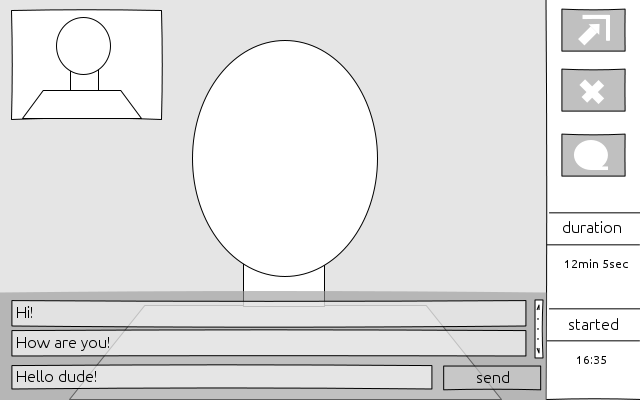
\includegraphics[height=0.6\textwidth]{../ui/img/uiDraft2/PhoneViewWithMessenger.png}
		\caption{Phone View: Nebst dem Video sieht der Benutzer elementare Informationen über den Anruf.}
		\label{settings screen}
	\end{figure}
	%	\begin{figure}[H]
	%	\centering
	%	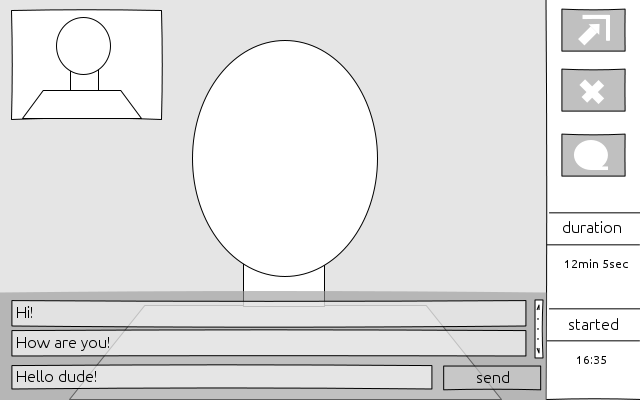
\includegraphics[height=0.6\textwidth]{../ui/img/uiDraft2/Phone view with messenger.png}
	%	\caption{Phone View: Nebst dem Video sieht der Benutzer elementare Informationen über den Anruf und kann dem andern Benutzer Nachrichten senden.}
	%	\label{settings screen}
	%\end{figure}
	\begin{figure}[H]
		\centering
		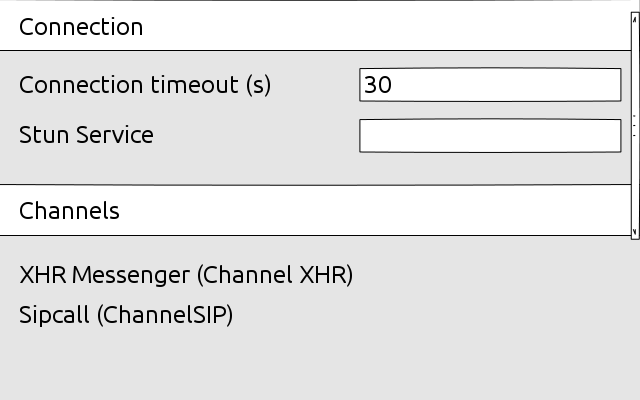
\includegraphics[height=0.6\textwidth]{../ui/img/uiDraft2/SettingsView.png}
		\caption{In den Settings kann der Benutzer Konfiguration und Channels einsehen.}
		\label{settings screen}
	\end{figure}
\end{landscape} 